% This file was created with tikzplotlib v0.10.1.
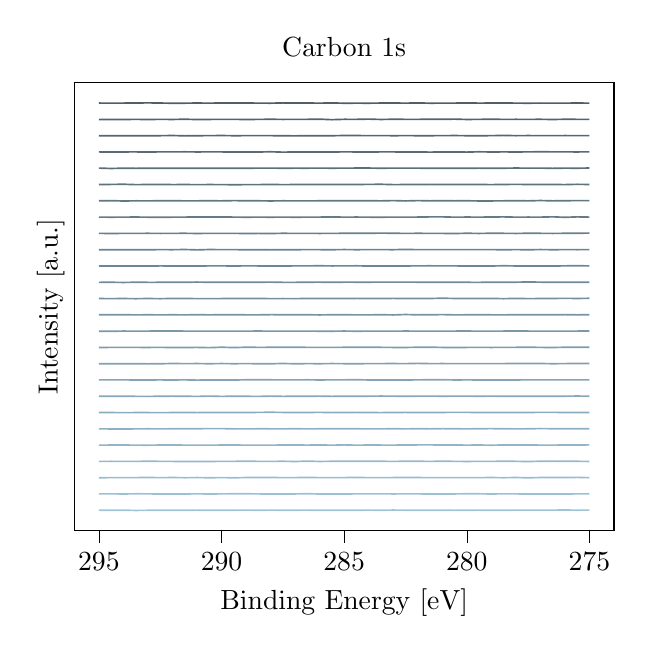
\begin{tikzpicture}

\definecolor{darkgray133164181}{RGB}{133,164,181}
\definecolor{darkgray136168186}{RGB}{136,168,186}
\definecolor{darkgray139172190}{RGB}{139,172,190}
\definecolor{darkgray143176195}{RGB}{143,176,195}
\definecolor{darkgray146180200}{RGB}{146,180,200}
\definecolor{darkgray176}{RGB}{176,176,176}
\definecolor{dimgray7895105}{RGB}{78,95,105}
\definecolor{dimgray8199110}{RGB}{81,99,110}
\definecolor{dimgray84103114}{RGB}{84,103,114}
\definecolor{dimgray88107118}{RGB}{88,107,118}
\definecolor{dimgray91111123}{RGB}{91,111,123}
\definecolor{lightslategray114139154}{RGB}{114,139,154}
\definecolor{lightslategray117143159}{RGB}{117,143,159}
\definecolor{lightslategray120147163}{RGB}{120,147,163}
\definecolor{lightslategray123152168}{RGB}{123,152,168}
\definecolor{lightslategray126156172}{RGB}{126,156,172}
\definecolor{lightslategray130160177}{RGB}{130,160,177}
\definecolor{lightsteelblue149184204}{RGB}{149,184,204}
\definecolor{lightsteelblue152188209}{RGB}{152,188,209}
\definecolor{lightsteelblue156192213}{RGB}{156,192,213}
\definecolor{lightsteelblue159196218}{RGB}{159,196,218}
\definecolor{slategray101123137}{RGB}{101,123,137}
\definecolor{slategray104127141}{RGB}{104,127,141}
\definecolor{slategray107131146}{RGB}{107,131,146}
\definecolor{slategray110135150}{RGB}{110,135,150}
\definecolor{slategray94115128}{RGB}{94,115,128}
\definecolor{slategray97119132}{RGB}{97,119,132}

\begin{axis}[
scaled y ticks=manual:{}{\pgfmathparse{#1}},
tick align=outside,
title={Carbon 1s},
x dir=reverse,
x grid style={darkgray176},
xlabel={Binding Energy [eV]},
xmin=274, xmax=296,
xtick pos=left,
xtick style={color=black},
y grid style={darkgray176},
ylabel={Intensity [a.u.]},
ymajorticks=false,
ymin=-130563.4, ymax=7099.4,
ytick style={color=black},
yticklabels={}
]
\addplot [semithick, dimgray7895105]
table {%
295 780
294.5 762
294 776
293.5 799
293 842
292.5 791
292 728
291.5 747
291 796
290.5 751
290 819
289.5 804
289 789
288.5 771
288 744
287.5 828
287 799
286.5 802
286 756
285.5 826
285 734
284.5 757
284 742
283.5 785
283 806
282.5 757
282 828
281.5 740
281 767
280.5 772
280 819
279.5 768
279 790
278.5 818
278 765
277.5 739
277 778
276.5 764
276 753
275.5 804
275 751
};
\addplot [semithick, dimgray8199110]
table {%
295 -4291
294.5 -4245
294 -4271
293.5 -4219
293 -4277
292.5 -4216
292 -4251
291.5 -4179
291 -4280
290.5 -4241
290 -4232
289.5 -4230
289 -4251
288.5 -4235
288 -4189
287.5 -4241
287 -4226
286.5 -4214
286 -4167
285.5 -4320
285 -4211
284.5 -4216
284 -4149
283.5 -4252
283 -4186
282.5 -4217
282 -4218
281.5 -4187
281 -4197
280.5 -4154
280 -4253
279.5 -4222
279 -4177
278.5 -4228
278 -4211
277.5 -4222
277 -4206
276.5 -4266
276 -4193
275.5 -4215
275 -4213
};
\addplot [semithick, dimgray84103114]
table {%
295 -9263
294.5 -9234
294 -9265
293.5 -9256
293 -9238
292.5 -9232
292 -9182
291.5 -9282
291 -9238
290.5 -9221
290 -9185
289.5 -9242
289 -9221
288.5 -9221
288 -9223
287.5 -9256
287 -9289
286.5 -9232
286 -9241
285.5 -9249
285 -9181
284.5 -9199
284 -9207
283.5 -9207
283 -9237
282.5 -9219
282 -9234
281.5 -9231
281 -9226
280.5 -9190
280 -9239
279.5 -9233
279 -9228
278.5 -9150
278 -9231
277.5 -9197
277 -9226
276.5 -9217
276 -9201
275.5 -9209
275 -9205
};
\addplot [semithick, dimgray88107118]
table {%
295 -14218
294.5 -14232
294 -14223
293.5 -14214
293 -14258
292.5 -14203
292 -14205
291.5 -14189
291 -14225
290.5 -14206
290 -14214
289.5 -14265
289 -14231
288.5 -14252
288 -14166
287.5 -14292
287 -14228
286.5 -14256
286 -14222
285.5 -14268
285 -14191
284.5 -14233
284 -14230
283.5 -14217
283 -14215
282.5 -14242
282 -14226
281.5 -14280
281 -14229
280.5 -14237
280 -14272
279.5 -14180
279 -14242
278.5 -14209
278 -14236
277.5 -14205
277 -14176
276.5 -14198
276 -14208
275.5 -14224
275 -14192
};
\addplot [semithick, dimgray91111123]
table {%
295 -19191
294.5 -19302
294 -19213
293.5 -19259
293 -19246
292.5 -19234
292 -19236
291.5 -19232
291 -19227
290.5 -19222
290 -19249
289.5 -19226
289 -19227
288.5 -19200
288 -19194
287.5 -19220
287 -19207
286.5 -19212
286 -19185
285.5 -19220
285 -19191
284.5 -19179
284 -19173
283.5 -19237
283 -19184
282.5 -19193
282 -19201
281.5 -19240
281 -19213
280.5 -19209
280 -19252
279.5 -19204
279 -19256
278.5 -19221
278 -19170
277.5 -19210
277 -19182
276.5 -19261
276 -19199
275.5 -19224
275 -19163
};
\addplot [semithick, slategray94115128]
table {%
295 -24236
294.5 -24197
294 -24145
293.5 -24264
293 -24229
292.5 -24211
292 -24253
291.5 -24238
291 -24261
290.5 -24244
290 -24255
289.5 -24292
289 -24267
288.5 -24259
288 -24208
287.5 -24266
287 -24233
286.5 -24218
286 -24235
285.5 -24204
285 -24216
284.5 -24218
284 -24186
283.5 -24156
283 -24258
282.5 -24239
282 -24234
281.5 -24198
281 -24205
280.5 -24235
280 -24246
279.5 -24230
279 -24256
278.5 -24221
278 -24172
277.5 -24223
277 -24211
276.5 -24228
276 -24255
275.5 -24168
275 -24221
};
\addplot [semithick, slategray97119132]
table {%
295 -29231
294.5 -29187
294 -29290
293.5 -29236
293 -29248
292.5 -29221
292 -29229
291.5 -29240
291 -29239
290.5 -29231
290 -29240
289.5 -29177
289 -29213
288.5 -29229
288 -29275
287.5 -29233
287 -29254
286.5 -29249
286 -29234
285.5 -29219
285 -29215
284.5 -29214
284 -29205
283.5 -29246
283 -29167
282.5 -29267
282 -29169
281.5 -29241
281 -29199
280.5 -29239
280 -29220
279.5 -29274
279 -29270
278.5 -29237
278 -29197
277.5 -29243
277 -29149
276.5 -29241
276 -29213
275.5 -29163
275 -29183
};
\addplot [semithick, slategray101123137]
table {%
295 -34240
294.5 -34261
294 -34242
293.5 -34214
293 -34258
292.5 -34263
292 -34254
291.5 -34231
291 -34208
290.5 -34188
290 -34196
289.5 -34232
289 -34270
288.5 -34239
288 -34264
287.5 -34235
287 -34267
286.5 -34244
286 -34233
285.5 -34176
285 -34248
284.5 -34223
284 -34253
283.5 -34267
283 -34228
282.5 -34248
282 -34226
281.5 -34172
281 -34164
280.5 -34255
280 -34220
279.5 -34243
279 -34203
278.5 -34169
278 -34249
277.5 -34226
277 -34240
276.5 -34152
276 -34295
275.5 -34167
275 -34236
};
\addplot [semithick, slategray104127141]
table {%
295 -39232
294.5 -39260
294 -39235
293.5 -39234
293 -39213
292.5 -39245
292 -39227
291.5 -39209
291 -39263
290.5 -39219
290 -39224
289.5 -39224
289 -39271
288.5 -39242
288 -39271
287.5 -39207
287 -39235
286.5 -39232
286 -39246
285.5 -39233
285 -39206
284.5 -39170
284 -39207
283.5 -39146
283 -39191
282.5 -39237
282 -39210
281.5 -39229
281 -39239
280.5 -39279
280 -39193
279.5 -39250
279 -39191
278.5 -39216
278 -39248
277.5 -39194
277 -39216
276.5 -39246
276 -39207
275.5 -39198
275 -39137
};
\addplot [semithick, slategray107131146]
table {%
295 -44239
294.5 -44236
294 -44271
293.5 -44253
293 -44256
292.5 -44222
292 -44239
291.5 -44187
291 -44296
290.5 -44189
290 -44225
289.5 -44215
289 -44270
288.5 -44244
288 -44285
287.5 -44245
287 -44251
286.5 -44215
286 -44233
285.5 -44248
285 -44202
284.5 -44243
284 -44213
283.5 -44218
283 -44241
282.5 -44156
282 -44233
281.5 -44222
281 -44215
280.5 -44210
280 -44233
279.5 -44233
279 -44215
278.5 -44266
278 -44218
277.5 -44265
277 -44203
276.5 -44249
276 -44218
275.5 -44235
275 -44226
};
\addplot [semithick, slategray110135150]
table {%
295 -49275
294.5 -49234
294 -49243
293.5 -49255
293 -49269
292.5 -49218
292 -49246
291.5 -49230
291 -49257
290.5 -49215
290 -49203
289.5 -49260
289 -49197
288.5 -49226
288 -49238
287.5 -49240
287 -49219
286.5 -49208
286 -49182
285.5 -49225
285 -49217
284.5 -49192
284 -49261
283.5 -49244
283 -49240
282.5 -49236
282 -49206
281.5 -49193
281 -49224
280.5 -49213
280 -49255
279.5 -49273
279 -49244
278.5 -49179
278 -49234
277.5 -49254
277 -49240
276.5 -49262
276 -49204
275.5 -49160
275 -49226
};
\addplot [semithick, lightslategray114139154]
table {%
295 -54266
294.5 -54247
294 -54300
293.5 -54238
293 -54265
292.5 -54262
292 -54218
291.5 -54261
291 -54183
290.5 -54244
290 -54231
289.5 -54219
289 -54215
288.5 -54237
288 -54198
287.5 -54266
287 -54267
286.5 -54225
286 -54207
285.5 -54259
285 -54209
284.5 -54215
284 -54217
283.5 -54204
283 -54213
282.5 -54196
282 -54216
281.5 -54236
281 -54234
280.5 -54231
280 -54259
279.5 -54272
279 -54217
278.5 -54243
278 -54225
277.5 -54139
277 -54213
276.5 -54234
276 -54235
275.5 -54235
275 -54234
};
\addplot [semithick, lightslategray117143159]
table {%
295 -59243
294.5 -59266
294 -59238
293.5 -59285
293 -59234
292.5 -59283
292 -59221
291.5 -59238
291 -59260
290.5 -59257
290 -59253
289.5 -59217
289 -59224
288.5 -59229
288 -59264
287.5 -59252
287 -59281
286.5 -59210
286 -59209
285.5 -59235
285 -59247
284.5 -59203
284 -59207
283.5 -59252
283 -59198
282.5 -59250
282 -59216
281.5 -59226
281 -59139
280.5 -59217
280 -59218
279.5 -59249
279 -59203
278.5 -59283
278 -59203
277.5 -59267
277 -59243
276.5 -59220
276 -59180
275.5 -59218
275 -59168
};
\addplot [semithick, lightslategray120147163]
table {%
295 -64204
294.5 -64207
294 -64202
293.5 -64266
293 -64223
292.5 -64266
292 -64230
291.5 -64262
291 -64210
290.5 -64255
290 -64214
289.5 -64212
289 -64245
288.5 -64250
288 -64190
287.5 -64205
287 -64224
286.5 -64219
286 -64274
285.5 -64221
285 -64217
284.5 -64260
284 -64261
283.5 -64213
283 -64273
282.5 -64150
282 -64244
281.5 -64229
281 -64176
280.5 -64254
280 -64238
279.5 -64195
279 -64243
278.5 -64258
278 -64203
277.5 -64196
277 -64234
276.5 -64228
276 -64191
275.5 -64246
275 -64214
};
\addplot [semithick, lightslategray123152168]
table {%
295 -69260
294.5 -69304
294 -69228
293.5 -69250
293 -69236
292.5 -69213
292 -69206
291.5 -69236
291 -69240
290.5 -69237
290 -69238
289.5 -69239
289 -69244
288.5 -69224
288 -69251
287.5 -69251
287 -69247
286.5 -69235
286 -69269
285.5 -69270
285 -69226
284.5 -69275
284 -69245
283.5 -69248
283 -69260
282.5 -69225
282 -69252
281.5 -69233
281 -69249
280.5 -69234
280 -69221
279.5 -69252
279 -69243
278.5 -69232
278 -69215
277.5 -69232
277 -69253
276.5 -69239
276 -69233
275.5 -69234
275 -69198
};
\addplot [semithick, lightslategray126156172]
table {%
295 -74287
294.5 -74236
294 -74241
293.5 -74247
293 -74253
292.5 -74237
292 -74271
291.5 -74261
291 -74246
290.5 -74321
290 -74193
289.5 -74294
289 -74191
288.5 -74229
288 -74218
287.5 -74209
287 -74189
286.5 -74228
286 -74236
285.5 -74233
285 -74220
284.5 -74214
284 -74215
283.5 -74221
283 -74253
282.5 -74260
282 -74200
281.5 -74186
281 -74253
280.5 -74268
280 -74250
279.5 -74229
279 -74253
278.5 -74224
278 -74223
277.5 -74184
277 -74242
276.5 -74272
276 -74201
275.5 -74214
275 -74197
};
\addplot [semithick, lightslategray130160177]
table {%
295 -79263
294.5 -79248
294 -79246
293.5 -79272
293 -79291
292.5 -79266
292 -79185
291.5 -79233
291 -79205
290.5 -79257
290 -79206
289.5 -79251
289 -79216
288.5 -79261
288 -79272
287.5 -79185
287 -79269
286.5 -79229
286 -79249
285.5 -79207
285 -79242
284.5 -79256
284 -79227
283.5 -79215
283 -79206
282.5 -79227
282 -79153
281.5 -79224
281 -79209
280.5 -79235
280 -79217
279.5 -79223
279 -79235
278.5 -79213
278 -79204
277.5 -79191
277 -79188
276.5 -79254
276 -79215
275.5 -79192
275 -79177
};
\addplot [semithick, darkgray133164181]
table {%
295 -84221
294.5 -84216
294 -84207
293.5 -84251
293 -84238
292.5 -84225
292 -84245
291.5 -84213
291 -84286
290.5 -84247
290 -84249
289.5 -84264
289 -84187
288.5 -84197
288 -84199
287.5 -84228
287 -84223
286.5 -84196
286 -84247
285.5 -84205
285 -84207
284.5 -84164
284 -84243
283.5 -84252
283 -84276
282.5 -84260
282 -84209
281.5 -84186
281 -84180
280.5 -84238
280 -84222
279.5 -84237
279 -84256
278.5 -84237
278 -84237
277.5 -84215
277 -84218
276.5 -84203
276 -84211
275.5 -84210
275 -84222
};
\addplot [semithick, darkgray136168186]
table {%
295 -89233
294.5 -89258
294 -89222
293.5 -89271
293 -89296
292.5 -89235
292 -89216
291.5 -89238
291 -89294
290.5 -89195
290 -89283
289.5 -89236
289 -89256
288.5 -89289
288 -89209
287.5 -89275
287 -89242
286.5 -89248
286 -89211
285.5 -89270
285 -89251
284.5 -89263
284 -89216
283.5 -89188
283 -89212
282.5 -89246
282 -89211
281.5 -89202
281 -89231
280.5 -89205
280 -89208
279.5 -89229
279 -89212
278.5 -89227
278 -89239
277.5 -89231
277 -89232
276.5 -89251
276 -89223
275.5 -89182
275 -89226
};
\addplot [semithick, darkgray139172190]
table {%
295 -94229
294.5 -94246
294 -94284
293.5 -94253
293 -94256
292.5 -94285
292 -94249
291.5 -94236
291 -94260
290.5 -94228
290 -94226
289.5 -94219
289 -94249
288.5 -94199
288 -94162
287.5 -94210
287 -94218
286.5 -94232
286 -94188
285.5 -94259
285 -94213
284.5 -94208
284 -94232
283.5 -94266
283 -94217
282.5 -94207
282 -94238
281.5 -94257
281 -94220
280.5 -94181
280 -94201
279.5 -94225
279 -94256
278.5 -94228
278 -94239
277.5 -94229
277 -94192
276.5 -94188
276 -94234
275.5 -94219
275 -94258
};
\addplot [semithick, darkgray143176195]
table {%
295 -99247
294.5 -99284
294 -99300
293.5 -99267
293 -99242
292.5 -99271
292 -99236
291.5 -99243
291 -99207
290.5 -99189
290 -99177
289.5 -99251
289 -99271
288.5 -99241
288 -99248
287.5 -99271
287 -99209
286.5 -99271
286 -99236
285.5 -99213
285 -99228
284.5 -99246
284 -99250
283.5 -99264
283 -99222
282.5 -99261
282 -99225
281.5 -99252
281 -99195
280.5 -99225
280 -99265
279.5 -99217
279 -99191
278.5 -99240
278 -99252
277.5 -99246
277 -99169
276.5 -99212
276 -99219
275.5 -99201
275 -99247
};
\addplot [semithick, darkgray146180200]
table {%
295 -104260
294.5 -104230
294 -104214
293.5 -104259
293 -104270
292.5 -104226
292 -104208
291.5 -104246
291 -104259
290.5 -104246
290 -104234
289.5 -104230
289 -104243
288.5 -104249
288 -104245
287.5 -104230
287 -104215
286.5 -104245
286 -104200
285.5 -104263
285 -104183
284.5 -104265
284 -104218
283.5 -104237
283 -104243
282.5 -104222
282 -104186
281.5 -104172
281 -104235
280.5 -104214
280 -104248
279.5 -104218
279 -104277
278.5 -104198
278 -104201
277.5 -104212
277 -104244
276.5 -104255
276 -104213
275.5 -104234
275 -104170
};
\addplot [semithick, lightsteelblue149184204]
table {%
295 -109254
294.5 -109226
294 -109247
293.5 -109250
293 -109197
292.5 -109235
292 -109249
291.5 -109296
291 -109254
290.5 -109282
290 -109227
289.5 -109236
289 -109190
288.5 -109234
288 -109248
287.5 -109214
287 -109279
286.5 -109175
286 -109263
285.5 -109217
285 -109216
284.5 -109221
284 -109200
283.5 -109214
283 -109248
282.5 -109202
282 -109212
281.5 -109239
281 -109202
280.5 -109232
280 -109265
279.5 -109228
279 -109250
278.5 -109190
278 -109228
277.5 -109284
277 -109202
276.5 -109176
276 -109223
275.5 -109220
275 -109260
};
\addplot [semithick, lightsteelblue152188209]
table {%
295 -114268
294.5 -114231
294 -114243
293.5 -114228
293 -114185
292.5 -114244
292 -114200
291.5 -114248
291 -114214
290.5 -114267
290 -114221
289.5 -114272
289 -114208
288.5 -114208
288 -114210
287.5 -114221
287 -114223
286.5 -114193
286 -114224
285.5 -114241
285 -114223
284.5 -114183
284 -114234
283.5 -114242
283 -114216
282.5 -114196
282 -114209
281.5 -114237
281 -114230
280.5 -114240
280 -114220
279.5 -114238
279 -114201
278.5 -114251
278 -114197
277.5 -114281
277 -114201
276.5 -114193
276 -114213
275.5 -114159
275 -114248
};
\addplot [semithick, lightsteelblue156192213]
table {%
295 -119227
294.5 -119208
294 -119254
293.5 -119200
293 -119211
292.5 -119284
292 -119242
291.5 -119263
291 -119203
290.5 -119266
290 -119219
289.5 -119193
289 -119187
288.5 -119227
288 -119268
287.5 -119263
287 -119236
286.5 -119177
286 -119254
285.5 -119243
285 -119263
284.5 -119221
284 -119212
283.5 -119210
283 -119239
282.5 -119212
282 -119226
281.5 -119252
281 -119241
280.5 -119238
280 -119185
279.5 -119203
279 -119254
278.5 -119210
278 -119226
277.5 -119266
277 -119235
276.5 -119262
276 -119266
275.5 -119219
275 -119205
};
\addplot [semithick, lightsteelblue159196218]
table {%
295 -124220
294.5 -124254
294 -124231
293.5 -124306
293 -124270
292.5 -124251
292 -124257
291.5 -124228
291 -124223
290.5 -124233
290 -124224
289.5 -124239
289 -124199
288.5 -124251
288 -124206
287.5 -124254
287 -124239
286.5 -124207
286 -124272
285.5 -124225
285 -124237
284.5 -124271
284 -124206
283.5 -124245
283 -124191
282.5 -124228
282 -124225
281.5 -124259
281 -124253
280.5 -124274
280 -124233
279.5 -124220
279 -124262
278.5 -124243
278 -124217
277.5 -124206
277 -124201
276.5 -124213
276 -124170
275.5 -124228
275 -124204
};
\end{axis}

\end{tikzpicture}
